\section{Introduction}
\label{sec:intro}

Abstractive summarization is the task of creating a short, accurate,
informative and fluent summary from a longer text document.
It attempts to reproduce the semantics and topics of original text
by paraphrasing. 
Recently, sequence to sequence
models~\cite{RushCW15,ChopraAR16,NallapatiZSGX16,SeeLM17,PaulusXS17}
have made great progress on abstractive summarization.
Recent study~\cite{bai2018empirical} suggests that, 
without \DIFdelbegin \DIFdel{addtional}\DIFdelend \DIFaddbegin \DIFadd{additional}\DIFaddend , complicated structures or features,
convolutional sequence to sequence 
(CNN seq2seq) models~\cite{gehring2017convs2s,FanGA18,LiuLZ18} 
%CNN seq2seq models~\cite{gehring2017convs2s,FanGA18,LiuLZ18} 
%is a more powerful toolkit for sequence modeling than recurrent network.
are more effective and can be trained much faster due to 
its intrinsic parallel nature compared to recurrent networks (RNN).
Furthermore, unlike \DIFdelbegin \DIFdel{RNN }\DIFdelend \DIFaddbegin \DIFadd{RNN-based }\DIFaddend models, 
the convolutional models have more stable gradients 
because of its backpropagation paths. 
Thus, we take CNN seq2seq \DIFdelbegin \DIFdel{model }\DIFdelend \DIFaddbegin \DIFadd{models }\DIFaddend as the target model to improve on \DIFaddbegin \DIFadd{and
compare with
}\DIFaddend in this paper.

\DIFdelbegin \DIFdel{However}\DIFdelend \DIFaddbegin \DIFadd{Unfortunately}\DIFaddend , just like \DIFdelbegin \DIFdel{the RNN }\DIFdelend \DIFaddbegin \DIFadd{RNN-based }\DIFaddend models, CNN-based models \DIFdelbegin \DIFdel{often }\DIFdelend \DIFaddbegin \DIFadd{also }\DIFaddend produce
summaries with substantial repeated word sequences \DIFaddbegin \DIFadd{which impacts the reading efficiency}\DIFaddend .
\tabref{tab:example} illustrates one 
test case from the CNN/Daily Mail summarization dataset. 
In this case, the basic CNN produces two 
identical sentences (italized) in the result. 
Unlike machine translation or paraphrasing in which the output words
and input words are almost one-to-one aligned, the output of summarization
is ``compressed'' from the input document. Naturally, every sentence or 
word sequence in the summary corresponds to one or more places in the source
document. If there were two identical word sequences in the summary,
they might be looking at and summarizing the same ``spots'' in the source.
This is evident from the attention map for the three sentences generated by 
CNN, shown in \figref{fig:attn_map}. The 1st and 3rd \DIFdelbegin \DIFdel{sentence }\DIFdelend \DIFaddbegin \DIFadd{sentences }\DIFaddend attend to
the same location in the source (red boxes), while the second
sentence attends to another separate location in the source (green box). 
The two attention maps in the red boxes are very similar.

\DIFdelbegin %DIFDELCMD < \begin{table}[th]
%DIFDELCMD < %%%
\DIFdelendFL \DIFaddbeginFL \begin{table}[th!]
\DIFaddendFL \begin{center}
\scriptsize
\begin{tabular}{|l|}%{|p{7cm}|rl|}
\hline \bf Source document \\
\hline manchester city are rivalling manchester united and arsenal for valenciennes \\
       teenage defender dayot upamecano . the 16-year-old almost joined united in \\
	   the january transfer window only for him to opt to stay in france for a few \\
	   more months . centre-back umecano has played for france at u16 and u17 \\
	   level . monaco , inter milan and paris stgermain had also expressed interest. \\
	   fourth-placed city face aston villa at the etihad stadium on saturday . \\
\hline \bf Reference summary \\
\hline dayot upamecano was close to signing for manchester united in january . \\
       the 16-year-old, however , opted to stay in france with valenciennes . \\
	   centre-back upamecano has played for france at u16 and u17 level . \\
	   arsenal are also interested in the defender as man city join chase . \\
\hline \bf Basic CNN model (CNN) \\
\hline \textit{manchester city face aston villa at the etihad stadium on saturday .}\\
       the 16-year-old almost joined united in the january transfer window . \\
	   \textit{manchester city face aston villa at the etihad stadium on saturday .}\\
\hline
\end{tabular}
\end{center}
\caption{\label{tab:example} Summary generated by the basic CNN model}
\end{table}


\begin{figure}[th!]
\centering
\subfigure[Attention distribution]{
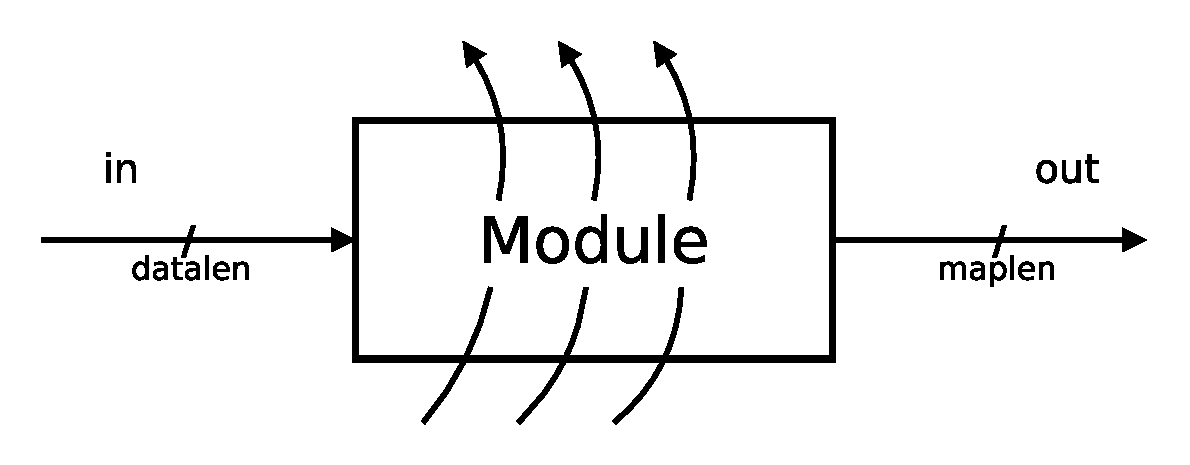
\includegraphics[width=0.8\linewidth]{map}
}
\quad
\subfigure[Green box]{
\includegraphics[width=0.44\linewidth]{map_1}
}
\quad
\subfigure[Red box]{
\includegraphics[width=0.44\linewidth]{map_2}
}
\caption{Attention for example on CNN model in \tabref{tab:example}}
\label{fig:attn_map}
\end{figure}

Driven by this intuition, a few efforts have been made on ``remembering''
what has been focused on before at decoding. 
For example, 
Paulus~\DIFdelbegin %DIFDELCMD < \shortcite{PaulusXS17} %%%
\DIFdelend \DIFaddbegin \DIFadd{\mbox{%DIFAUXCMD
\cite{PaulusXS17} }\hspace{0pt}%DIFAUXCMD
}\DIFaddend and 
Fan~\DIFdelbegin %DIFDELCMD < \shortcite{FanGA18} %%%
\DIFdelend \DIFaddbegin \DIFadd{\mbox{%DIFAUXCMD
\cite{FanGA18} }\hspace{0pt}%DIFAUXCMD
}\DIFaddend use intra-temporal 
attention~\cite{NallapatiZSGX16} as well as intra-decoder attention to avoid
attending to the same parts in the source by 
revising attention scores while decoding. 
See~\DIFdelbegin %DIFDELCMD < \shortcite{SeeLM17} %%%
\DIFdelend \DIFaddbegin \DIFadd{\mbox{%DIFAUXCMD
\cite{SeeLM17} }\hspace{0pt}%DIFAUXCMD
}\DIFaddend and Gehrmann~\DIFdelbegin %DIFDELCMD < \shortcite{GehrmannDR18}
%DIFDELCMD < %%%
\DIFdelend \DIFaddbegin \DIFadd{\mbox{%DIFAUXCMD
\cite{GehrmannDR18}
}\hspace{0pt}%DIFAUXCMD
}\DIFaddend respectively propose coverage mechanism and coverage penalty,
which \DIFdelbegin \DIFdel{record }\DIFdelend \DIFaddbegin \DIFadd{records }\DIFaddend the sum of attention distributions of all previously generated words 
%to keep track of what has been summarized in different way.  
in \DIFaddbegin \DIFadd{a }\DIFaddend different way to track the summarized information.  
While these approaches discourage repetition to some extent,
they do so in an indirect manner\DIFdelbegin \DIFdel{, i.e. }\DIFdelend \DIFaddbegin \DIFadd{. That is}\DIFaddend , they do not 
make use of the attention information in source directly.
Consequently, they may still generate repeated phrases, 
especially in long sentences (shown in the first 5 sections of
\tabref{tab:strong_methods}).


\DIFdelbegin %DIFDELCMD < \begin{table}[th]
%DIFDELCMD < %%%
\DIFdelendFL \DIFaddbeginFL \begin{table}[th!]
\DIFaddendFL \begin{center}
\scriptsize
\begin{tabular}{|l|}%{|p{7cm}|rl|}

\hline \bf Intra-temporal attention (ITA) \\
\hline \textit{manchester city face aston villa at the etihad stadium on saturday .} \\
	   \textit{manchester city face aston villa at the etihad stadium on saturday .}\\
\hline \bf Intra-temporal $+$ Intra-decoder (ITDA) \\
\hline \textit{manchester city are rivalling manchester united and arsenal }for valenciennes\\
       teenage . manchester city face aston villa at the etihad stadium on saturday . \\
	   \textit{manchester city are rivalling manchester united and arsenal }. \\
\hline \bf Coverage model (COV) \\
\hline \textit{manchester city face aston villa at the etihad stadium on saturday .} \\
       manchester city are rivalling manchester united and arsenal for valenciennes . \\
	   \textit{manchester city face aston villa at the etihad stadium on saturday .}\\
\hline \bf Coverage penalty (COVP)\\
\hline \textit{manchester city face aston villa at the etihad stadium on saturday .}\\
       \textit{manchester city face aston villa at the etihad stadium on saturday .}\\
	   manchester city are rivalling manchester united and arsenal .\\
\hline \bf Semantic cohesion loss (SCL) \\
\hline \textit{manchester city are rivalling manchester united and arsenal for } defender \DIFdelbeginFL %DIFDELCMD < \\
%DIFDELCMD <        %%%
\DIFdelendFL dayot upamecano . \DIFaddbeginFL \\
       \DIFaddendFL \textit{manchester city are rivalling for} valenciennes teenage. \\
\hline \bf Trigram decoder (TRI) \\
\hline \underline{defender dayot upamecano} has played for \underline{france} at unk and unk level .\\ 
       manchester city face aston villa at the etihad stadium on saturday . \\
\hline \bf Ours (Attention Filter + Backtracking decoder) \\
\hline manchester city face aston villa at the etihad stadium on saturday . \\
       the 16-year-old almost joined united in the january transfer window . \\
	   manchester city are rivalling manchester united and arsenal for teenage \DIFdelbeginFL %DIFDELCMD < \\
%DIFDELCMD < 	   %%%
\DIFdelendFL defender daypot upamecano .\\
\hline
\end{tabular}
\end{center}
\caption{\label{tab:strong_methods} Generated summaries of the source in \tabref{tab:example}}
\end{table}

In this paper, we propose an attention filter mechanism that directly 
redistributes the attention from each word in the output summary to the source. 
It does so by computing the parts of interest (POIs) in the source
per segment in the summary~
\DIFdelbegin \footnote{\DIFdel{Segment means a sentence or clause delimited by punctuation.}}%DIFAUXCMD
\addtocounter{footnote}{-1}%DIFAUXCMD
\DIFdel{, 
}\DIFdelend %\footnote{In this paper, a segment means a sentence or clause delimited by punctuation.}, 
and then minimizing the attention scores of
words in these POIs that have already been attended to by the preceding 
segments during decoding. 
\DIFaddbegin \DIFadd{A segment means a sentence or clause delimited by punctuation,
which carries syntactic and semantic information. 
It is very simple but effective. Since punctuations 
play an important role in written language to organize 
the grammatical structures and to clarify the meaning of sentences~\mbox{%DIFAUXCMD
\cite{briscoe1996,Kim19,LiWE19}
}\hspace{0pt}%DIFAUXCMD
%DIF > (Jones, 1996;Briscoe et al., 1997;Kim et al., 2019;Li et al., 2019).
}\DIFaddend Specifically, we calculate the attention in terms of segments, larger semantic units than tokens, 
which intuitively helps with emphasis of attention and POIs in source.
Different segments in summary thus do not attend to the same semantic spots
of source, and repetition is reduced. 
This is different from previous approaches
which all do not exactly pinpoint these parts in the source,
which we believe is critical in reducing repetition. 
%This kind of partial attention 
%can help us to pinpoint the corresponding location that each segment is
%attending to. Then we use attention filter to filter
%a partial attention from normal attention of each tokens in the other sections
%by minimizing the attention scores of attended location in source document.
%This can optimize the alignment relationship between source document and 
%summarization.  This is shown in \tabref{tab:attn_exp}. 

Despite the above effort, there are cases, where similar sentences 
exist in the same source document:
\begin{example}
\label{ex:repeatsrc}
%\fbox{
%\parbox{0.9\columnwidth}{
\small{``..the standout fixture in the league on saturday sees leaders 
	   chelsea welcome manchester united ... chelsea midfielder oriol romeu, 
\textbf{currently on loan at stuttgart}, ... romeu is 
\textbf{currently on a season-long loan at bundesliga side stuttgart.}''} 
%}}
\end{example}

In this case, even if the decoder attends to different POIs of 
source document as it produces words, repetition may still result.  
At different timesteps,
the decoder may attend 
to sentences that are similar in different positions.
One potential solution to this is semantic cohesion loss~\cite{elikyilmazBHC18}
which takes the cosine similarity between two consecutively generated sentences
as part of the loss function. It may attend to the same POI
and generate similar sentences (SCL row in \tabref{tab:strong_methods}).  
The other is a trigram decoder~\cite{PaulusXS17} 
which directly forbids repetition of previously generated trigrams at test time. 
While this simple but crude method avoids the repeat of any kind
completely, 
it ignores the fact that \textit{some amount of repetition} may exist
in natural summaries.  
On the other hand, the meddling of the beam search at run-time causes another problem: 
it tends to generate sentences that are logically incorrect. 
In \tabref{tab:strong_methods} (TRI row), the defender dayot didn't
really play for France, according to the source.
That is, the subject and object are mismatched.
So in this paper, we instead introduce a {\em sentence-level} backtracking decoder
that prohibits the repeat of the same sentence \DIFdelbegin \DIFdel{during testing}\DIFdelend \DIFaddbegin \DIFadd{at test time}\DIFaddend .
Our summary produced for the example is shown in last section of 
\tabref{tab:strong_methods}.

%In multiple-sentence summarization task, we observe that more often than not, repetition 
%occurs in the form of the same or similar sentences, rather than repetitive phrases 
%inside sentences. 
%On the other hand, it is prone to grammatical and factual errors(\tabref{tab:attn_exp}).
%Because it detects repetitive trigrams only by setting the 
%probability of the third word to zero. 
%It ignores that there are some same N-gram in the target summaries.
%The natural generation of a sentence is disturbed, giving rise to, 
%for example, mismatch of subject and object, and wrong phrases. 
%summarization is not a text generation problem which are are almost
%one-to-one correspondence between input and output words, it requires the model 
%has the ability to decide where to attend and where to ignore.
%The reason for repetition in abstractive summarization based on CNN seq2seq models is
%that the models always attend to the same location in the source document.
%As shown \tabref{tab:attn_exp} 
%and \figref{fig:attn_map} are corresponding. 
%Sentence in blue has factual erro. and \figref{fig:attn_map}.
%In the attention map, the darker color, the higher attention score.
%the repeated sentence in summary attends to the same location
%with high attention score, and different sentences attend to different location in source document. 
%

%DIF < Zhou~\shortcite{ZhouYWZ17} pointed out that there is no obvious alignment relationship 
%DIF > Zhou~\cite{ZhouYWZ17} pointed out that there is no obvious alignment relationship 
%between the source text and the target summary, 
%and the encoder outputs contain noise for the attention. 
%Thus, removing repetition in abstractive summarization on CNN seq2seq model
%need a strong attention mechamism that can get alignment relationship
%between source document and target summary and determine the summarized
%parts in source documents directly. 

\DIFdelbegin %DIFDELCMD < \cut{%%%%%%%%%%%%%%%%
%DIFDELCMD < as shown in \tabref{tab:src_rep}.
%DIFDELCMD < \figref{fig:attn_map3} shows that the repeated sentences
%DIFDELCMD < in summary respectively attend to the similar sentences in source document.
%DIFDELCMD < So we force our decoder to never output the same sentence more than once by a sentence level
%DIFDELCMD < backtraching decoder during testing. 
%DIFDELCMD < 

%DIFDELCMD < \begin{table}[th!]
%DIFDELCMD < \begin{center}
%DIFDELCMD < \scriptsize
%DIFDELCMD < \begin{tabular}{lclclclc}%{|p{7cm}|rl|}
%DIFDELCMD < \hline \bf Source document \\
%DIFDELCMD < \hline chelsea 's on loan midfielder oriol romeu goes up against sportsmail 's \\
%DIFDELCMD <        martin ... . the standout fixture in the league on saturday sees leaders \\
%DIFDELCMD < 	   chelsea welcome manchester united to stamford bridge , ... \\
%DIFDELCMD < 	   chelsea midfielder oriol romeu , \textbf{currently on loan at stuttgart} , predicts \\
%DIFDELCMD < 	   the scores for the weekend 's matches . romeu is \textbf{currently on a season-long} \\
%DIFDELCMD < 	   \textbf{loan at bundesliga side stuttgart .} \\
%DIFDELCMD < \hline \bf Reference summary \\
%DIFDELCMD < \hline oriol romeu is on a season-long loan at stuttgart from chelsea . the spanish \\
%DIFDELCMD <        midfielder predicts the scores in saturday 's matches . romeu goes \\
%DIFDELCMD < 	   head-to-head with sportsmail 's martin keown . \\
%DIFDELCMD < \hline \bf Our (Attention Filter)\\
%DIFDELCMD < \hline chelsea beat manchester united on saturday . oriol romeu is currently \\
%DIFDELCMD <        on a season-long loan at stuttgart . oriol romeu is \\
%DIFDELCMD < 	   currently on a season-long loan at the end of the season .\\
%DIFDELCMD < \hline \bf Our (Attention Filter + Backtracking decoder) \\
%DIFDELCMD < \hline chelsea face manchester united in the premier league on saturday . oriol romeu \\
%DIFDELCMD <        is currently on loan at stuttgart . \\
%DIFDELCMD < \hline
%DIFDELCMD < \end{tabular}
%DIFDELCMD < \end{center}
%DIFDELCMD < \caption{\label{tab:src_rep} Summaries generated by source document with repeatedness. }
%DIFDELCMD < \end{table}
%DIFDELCMD < 

%DIFDELCMD < \begin{figure}[th!]
%DIFDELCMD < \centering
%DIFDELCMD < \includegraphics[width=0.9\linewidth]{map3}
%DIFDELCMD < \caption{Attention distribution(local) for our attention filter model in \tabref{tab:src_rep}}
%DIFDELCMD < \label{fig:attn_map3}
%DIFDELCMD < \end{figure}
%DIFDELCMD < }%%%
\DIFdelend \DIFaddbegin \cut{%%%%%%%%%%%%%%%%
as shown in \tabref{tab:src_rep}.
\figref{fig:attn_map3} shows that the repeated sentences
in summary respectively attend to the similar sentences in source document.
So we force our decoder to never output the same sentence more than once by a sentence level
backtraching decoder during testing. 

\begin{table}[th!]
\begin{center}
\small
\begin{tabular}{lclclclc}%{|p{7cm}|rl|}
\hline \bf Source document \\
\hline chelsea 's on loan midfielder oriol romeu goes up against sportsmail 's \\
       martin ... . the standout fixture in the league on saturday sees leaders \\
	   chelsea welcome manchester united to stamford bridge , ... \\
	   chelsea midfielder oriol romeu , \textbf{currently on loan at stuttgart} , predicts \\
	   the scores for the weekend 's matches . romeu is \textbf{currently on a season-long} \\
	   \textbf{loan at bundesliga side stuttgart .} \\
\hline \bf Reference summary \\
\hline oriol romeu is on a season-long loan at stuttgart from chelsea . the spanish \\
       midfielder predicts the scores in saturday 's matches . romeu goes \\
	   head-to-head with sportsmail 's martin keown . \\
\hline \bf Our (Attention Filter)\\
\hline chelsea beat manchester united on saturday . oriol romeu is currently \\
       on a season-long loan at stuttgart . oriol romeu is \\
	   currently on a season-long loan at the end of the season .\\
\hline \bf Our (Attention Filter + Backtracking decoder) \\
\hline chelsea face manchester united in the premier league on saturday . oriol romeu \\
       is currently on loan at stuttgart . \\
\hline
\end{tabular}
\end{center}
\caption{\label{tab:src_rep} Summaries generated by source document with repeatedness. }
\end{table}


\begin{figure}[th!]
\centering
\includegraphics[width=0.9\linewidth]{map3}
\caption{Attention distribution(local) for our attention filter model in \tabref{tab:src_rep}}
\label{fig:attn_map3}
\end{figure}
}\DIFaddend %%%%%%%%%%%%%%%%%%
%Compared with trigram decoder, we do not impact
%the process of beam search in the middle of a sentence, 
%which can reduce factual errors and grammatical erros(\tabref{tab:attn_exp}).

\DIFadd{Reducing repetition in abstractive summarization provides high-quality summaries for users and improves their reading efficiency.
We expect that other natural language generation (NLG) tasks with repetition problem can be enhances with our approach.}\DIFaddend
Our contributions are summarized as follows:
\begin{enumerate}
\item We identify the repetition problem in abstractive summaries generated
by CNN seq2seq models and \DIFaddbegin \DIFadd{find the reasons behind the repetition problem.
}\item \DIFadd{We }\DIFaddend propose new metrics to evaluate this problem\DIFaddbegin \DIFadd{: Repeatedness and Readability}\DIFaddend .
\item We propose an effective approach that redistributes attention scores 
during training time, and prevents repetition by sentence backtracking
at runtime to reduce repetition in CNN seq2seq model.
\item Our approach
outperforms the state-of-the-art (SOTA) CNN-based baselines 
%\KZ{Are those really SOTA methods? They are only SOTA CNN based methods, right?}
substantially by all evaluation metrics, including ROUGE scores, 
\DIFdelbegin \DIFdel{repetition }\DIFdelend \DIFaddbegin \DIFadd{repeatedness }\DIFaddend and readability.
\end{enumerate}

%Next, we present our approach based on convolutional sequence to sequence 
%model, followed by the evaluation of our approach and a discussion
%of related work. 
